\section*{Results}

\subsection*{Dataset description}
This \href{https://snap.stanford.edu/data/wikispeedia.html}{dataset} 
contains human navigation paths on Wikipedia, collected through the human-computation 
game Wikispeedia. In Wikispeedia, users are asked to navigate from a given source to a given 
target article, by only clicking Wikipedia links. A condensed version of Wikipedia (4,604 articles) is used. 

\subsubsection*{Data preparation}

The links.tsv file was used to analyze in Gephi as a preparation was done next actions:
\begin{itemize}
    \item header from file was deleted
    \item added source and target column names
    \item the sites identificators (nodes names) was url-decoded via python script available in 4.
\end{itemize}

\subsection*{Layout}

In figure \ref{fig_yifan} showed Yifan Hu laout for the graph. It can be seen the graph is divided into
2 weak connectivity components: the main one in the center and the component in the left that consists of 3 nodes that corresponds to articles: "Sponsorship Directdebit", "Directdebit", "Friend Directdebit".
As well as that it seen that nodes with low out-degree are force-pushed out of the other nodes.

\begin{center}
    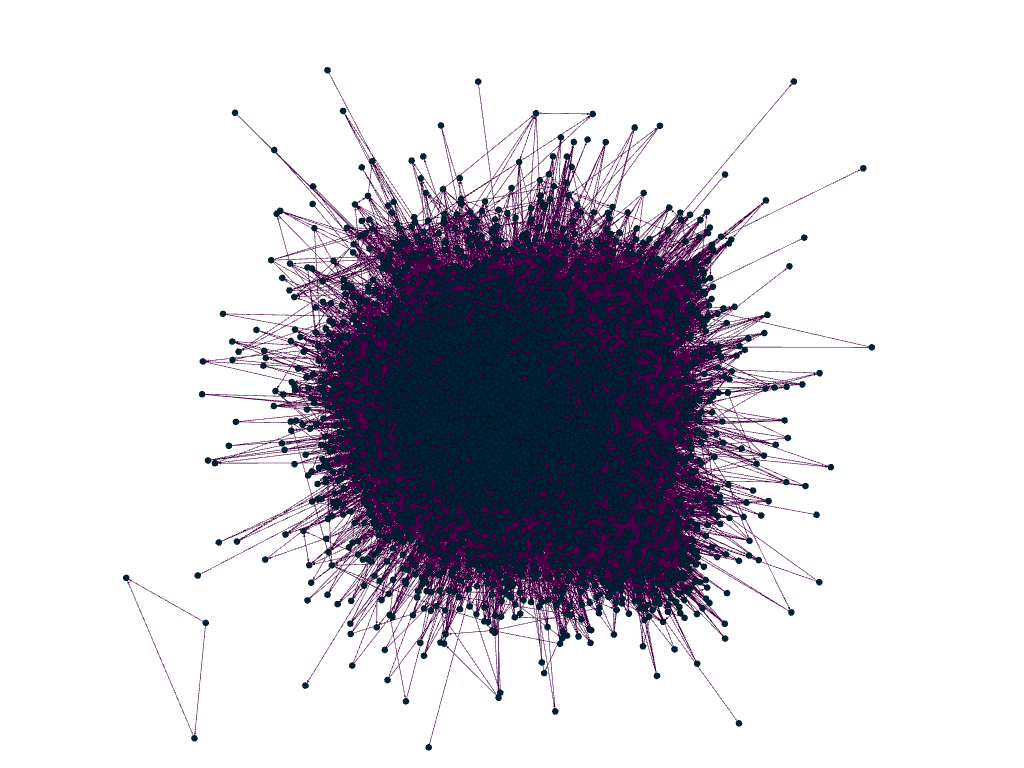
\includegraphics[width=0.75\linewidth]{../results/layout_1.png}
    \captionof{figure}{Yifan Hu layout of network}
    \label{fig_yifan}
\end{center}


In figure \ref{fig_atlas} showed Force atlas layout adjusted by sizes of nodes. Size for nodes was choosed according to their degrees. Used settings are showed in \ref{fig_settings}.

\begin{center}
    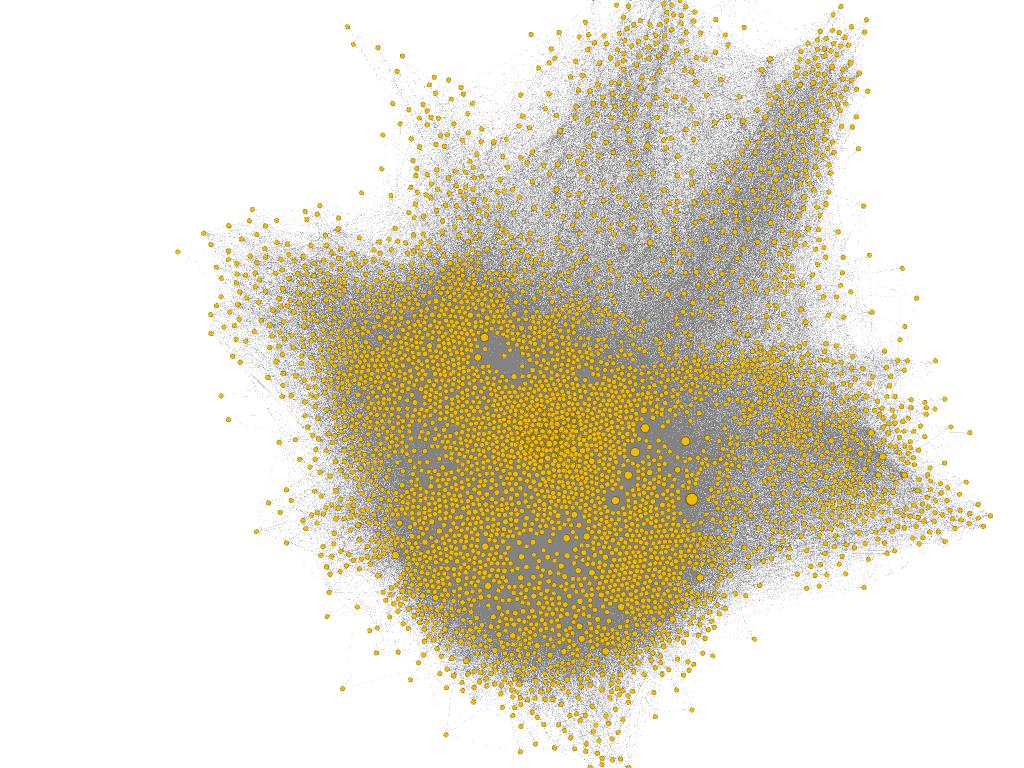
\includegraphics[width=0.75\linewidth]{../results/layout_3.png}
    \captionof{figure}{Force atlas adjasted by sizes of nodes due to its degrees}
    \label{fig_atlas}
\end{center}

\begin{center}
    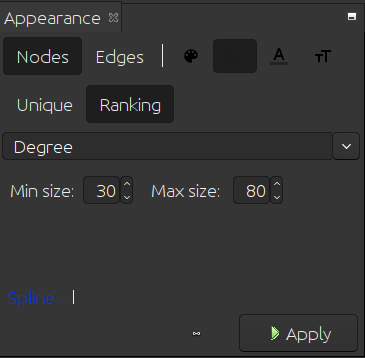
\includegraphics[width=0.4\linewidth]{../results/nodes_ranking.png}
    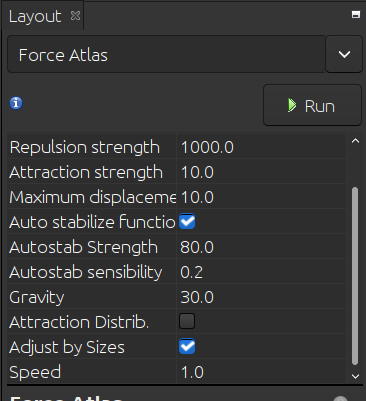
\includegraphics[width=0.4\linewidth]{../results/layout_settings.png}
    \captionof{figure}{Settings parameters for Force atlas laout}
    \label{fig_settings}
\end{center}

In figure \ref{fig_ord} the Open ord layout is shown along with grouping nodes according to modularity clustering with resolution of $0.9$. For example, the gray cluster corresponds to topics about animals, pink ones to computer connected articles (Windows XP, Internet explorer, Basic).

\begin{center}
    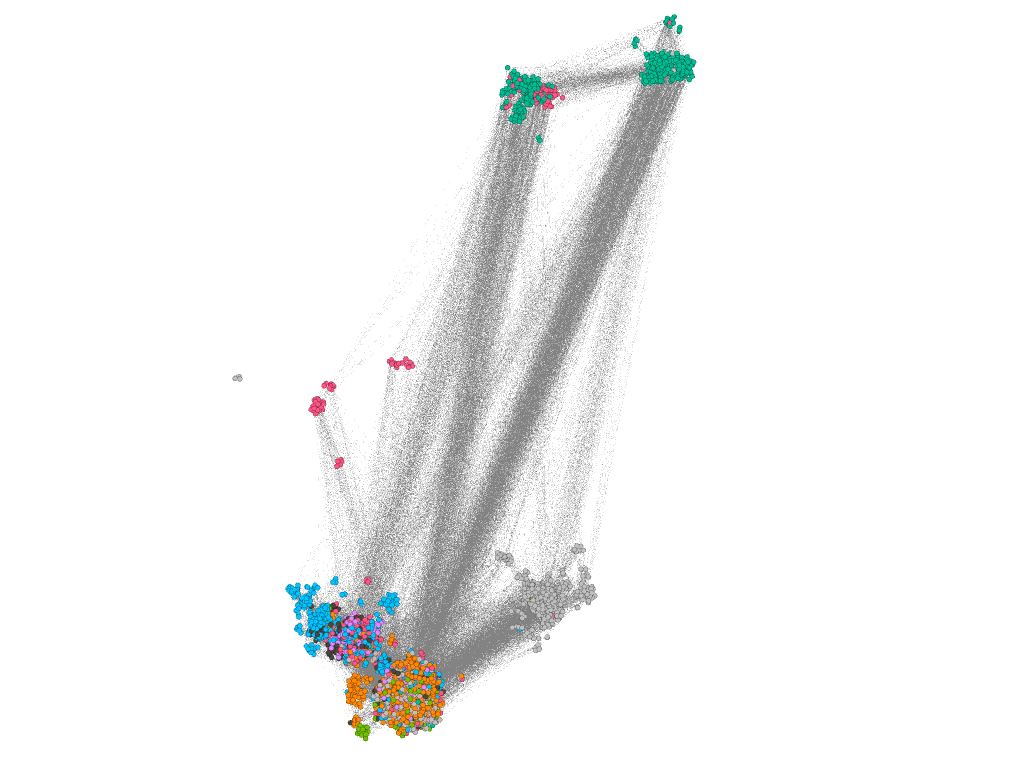
\includegraphics[width=0.75\linewidth]{../results/layout_2.png}
    \captionof{figure}{Open ord layout with modularity clustering}
    \label{fig_ord}
\end{center}

\subsection*{Network measures}

\textbf{The average degree} of vertices is \textbf{26} the distribution is shown in \ref{fig_degree_dist}.

\begin{center}
    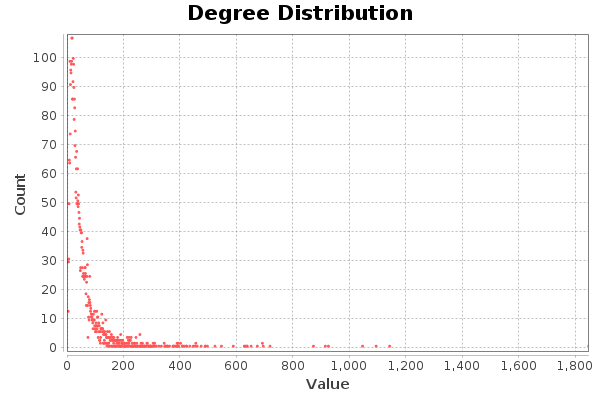
\includegraphics[width=0.75\linewidth]{../results/degree/degree-distribution.png}
    \captionof{figure}{Vertices degree distribution}
    \label{fig_degree_dist}
\end{center}

\textbf{D - the diameter of network} is \textbf{$9$}. It can be interpreted that playing in Wikispeedia the path person should do to go to target article is maximum 9 (if the target can be found from source target).

\textbf{Density $\rho$} = \textbf{0.006} - that means that graph can be considered as sparse.

After modularity clustering with resolution = 1 were obtained 8 clusters with distribution of nodes showed in \ref{fig_modularity} and overall modularity = \textbf{$0.366$}.

\begin{center}
    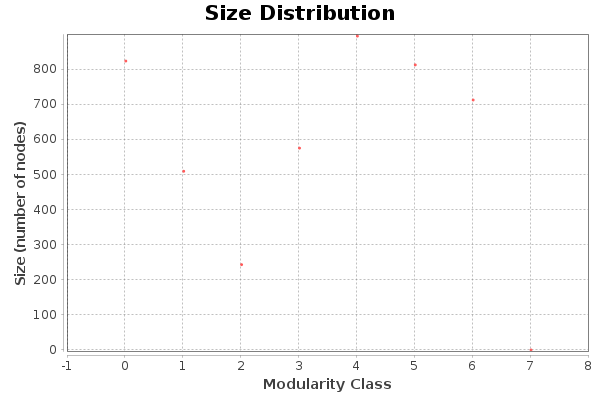
\includegraphics[width=0.75\linewidth]{../results/modularity_result/communities-size-distribution.png}
    \captionof{figure}{Clusters size distribution}
    \label{fig_modularity}
\end{center}

Some of obtained clusters can interpreted as follows: animals, computers, medicine and famous people. As it can be seen from \ref{fig_modularity} all clusters except one is quite large, the 7th cluster consist of only 3 vertices is the smallest weak connectivity component.

As well as 2 weakly connected components graph have 519 strongly connected component. That means that although we probably can have the path from one article to another there are cases when the reverse path does not exist. 

\subsubsection*{Nodes overview}

\textbf{Average Clustering Coefficient}: 0.183

\subsubsection*{Edge overview}

\textbf{Average path length:} 3.2. It can be interpreted as that if there is path from source article to target it usually takes 3 intermediate articles.

\subsection*{Conclusion}

From obtained results we can find next things:
\begin{itemize}
    \item Most of the articles are connected in one weakly component
    \item It takes up to 9 intermediate articles to reach the target article (if it is reachable)
    \item Clustering according to modularity can be representative in terms of topics of articles as they are divided in understandable communities with same subject.
\end{itemize}